\PassOptionsToPackage{unicode=true}{hyperref} % options for packages loaded elsewhere
\PassOptionsToPackage{hyphens}{url}
%
\documentclass[]{article}
\usepackage{lmodern}
\usepackage{amssymb,amsmath}
\usepackage{ifxetex,ifluatex}
\usepackage{fixltx2e} % provides \textsubscript
\ifnum 0\ifxetex 1\fi\ifluatex 1\fi=0 % if pdftex
  \usepackage[T1]{fontenc}
  \usepackage[utf8]{inputenc}
  \usepackage{textcomp} % provides euro and other symbols
\else % if luatex or xelatex
  \usepackage{unicode-math}
  \defaultfontfeatures{Ligatures=TeX,Scale=MatchLowercase}
\fi
% use upquote if available, for straight quotes in verbatim environments
\IfFileExists{upquote.sty}{\usepackage{upquote}}{}
% use microtype if available
\IfFileExists{microtype.sty}{%
\usepackage[]{microtype}
\UseMicrotypeSet[protrusion]{basicmath} % disable protrusion for tt fonts
}{}
\IfFileExists{parskip.sty}{%
\usepackage{parskip}
}{% else
\setlength{\parindent}{0pt}
\setlength{\parskip}{6pt plus 2pt minus 1pt}
}
\usepackage{hyperref}
\hypersetup{
            pdftitle={Assignment 1},
            pdfauthor={Group 1},
            pdfborder={0 0 0},
            breaklinks=true}
\urlstyle{same}  % don't use monospace font for urls
\usepackage[margin=1in]{geometry}
\usepackage{color}
\usepackage{fancyvrb}
\newcommand{\VerbBar}{|}
\newcommand{\VERB}{\Verb[commandchars=\\\{\}]}
\DefineVerbatimEnvironment{Highlighting}{Verbatim}{commandchars=\\\{\}}
% Add ',fontsize=\small' for more characters per line
\usepackage{framed}
\definecolor{shadecolor}{RGB}{248,248,248}
\newenvironment{Shaded}{\begin{snugshade}}{\end{snugshade}}
\newcommand{\AlertTok}[1]{\textcolor[rgb]{0.94,0.16,0.16}{#1}}
\newcommand{\AnnotationTok}[1]{\textcolor[rgb]{0.56,0.35,0.01}{\textbf{\textit{#1}}}}
\newcommand{\AttributeTok}[1]{\textcolor[rgb]{0.77,0.63,0.00}{#1}}
\newcommand{\BaseNTok}[1]{\textcolor[rgb]{0.00,0.00,0.81}{#1}}
\newcommand{\BuiltInTok}[1]{#1}
\newcommand{\CharTok}[1]{\textcolor[rgb]{0.31,0.60,0.02}{#1}}
\newcommand{\CommentTok}[1]{\textcolor[rgb]{0.56,0.35,0.01}{\textit{#1}}}
\newcommand{\CommentVarTok}[1]{\textcolor[rgb]{0.56,0.35,0.01}{\textbf{\textit{#1}}}}
\newcommand{\ConstantTok}[1]{\textcolor[rgb]{0.00,0.00,0.00}{#1}}
\newcommand{\ControlFlowTok}[1]{\textcolor[rgb]{0.13,0.29,0.53}{\textbf{#1}}}
\newcommand{\DataTypeTok}[1]{\textcolor[rgb]{0.13,0.29,0.53}{#1}}
\newcommand{\DecValTok}[1]{\textcolor[rgb]{0.00,0.00,0.81}{#1}}
\newcommand{\DocumentationTok}[1]{\textcolor[rgb]{0.56,0.35,0.01}{\textbf{\textit{#1}}}}
\newcommand{\ErrorTok}[1]{\textcolor[rgb]{0.64,0.00,0.00}{\textbf{#1}}}
\newcommand{\ExtensionTok}[1]{#1}
\newcommand{\FloatTok}[1]{\textcolor[rgb]{0.00,0.00,0.81}{#1}}
\newcommand{\FunctionTok}[1]{\textcolor[rgb]{0.00,0.00,0.00}{#1}}
\newcommand{\ImportTok}[1]{#1}
\newcommand{\InformationTok}[1]{\textcolor[rgb]{0.56,0.35,0.01}{\textbf{\textit{#1}}}}
\newcommand{\KeywordTok}[1]{\textcolor[rgb]{0.13,0.29,0.53}{\textbf{#1}}}
\newcommand{\NormalTok}[1]{#1}
\newcommand{\OperatorTok}[1]{\textcolor[rgb]{0.81,0.36,0.00}{\textbf{#1}}}
\newcommand{\OtherTok}[1]{\textcolor[rgb]{0.56,0.35,0.01}{#1}}
\newcommand{\PreprocessorTok}[1]{\textcolor[rgb]{0.56,0.35,0.01}{\textit{#1}}}
\newcommand{\RegionMarkerTok}[1]{#1}
\newcommand{\SpecialCharTok}[1]{\textcolor[rgb]{0.00,0.00,0.00}{#1}}
\newcommand{\SpecialStringTok}[1]{\textcolor[rgb]{0.31,0.60,0.02}{#1}}
\newcommand{\StringTok}[1]{\textcolor[rgb]{0.31,0.60,0.02}{#1}}
\newcommand{\VariableTok}[1]{\textcolor[rgb]{0.00,0.00,0.00}{#1}}
\newcommand{\VerbatimStringTok}[1]{\textcolor[rgb]{0.31,0.60,0.02}{#1}}
\newcommand{\WarningTok}[1]{\textcolor[rgb]{0.56,0.35,0.01}{\textbf{\textit{#1}}}}
\usepackage{graphicx,grffile}
\makeatletter
\def\maxwidth{\ifdim\Gin@nat@width>\linewidth\linewidth\else\Gin@nat@width\fi}
\def\maxheight{\ifdim\Gin@nat@height>\textheight\textheight\else\Gin@nat@height\fi}
\makeatother
% Scale images if necessary, so that they will not overflow the page
% margins by default, and it is still possible to overwrite the defaults
% using explicit options in \includegraphics[width, height, ...]{}
\setkeys{Gin}{width=\maxwidth,height=\maxheight,keepaspectratio}
\setlength{\emergencystretch}{3em}  % prevent overfull lines
\providecommand{\tightlist}{%
  \setlength{\itemsep}{0pt}\setlength{\parskip}{0pt}}
\setcounter{secnumdepth}{0}
% Redefines (sub)paragraphs to behave more like sections
\ifx\paragraph\undefined\else
\let\oldparagraph\paragraph
\renewcommand{\paragraph}[1]{\oldparagraph{#1}\mbox{}}
\fi
\ifx\subparagraph\undefined\else
\let\oldsubparagraph\subparagraph
\renewcommand{\subparagraph}[1]{\oldsubparagraph{#1}\mbox{}}
\fi

% set default figure placement to htbp
\makeatletter
\def\fps@figure{htbp}
\makeatother


\title{Assignment 1}
\author{Group 1}
\date{November 22th, 2020}

\begin{document}
\maketitle

Importing libraries

\begin{Shaded}
\begin{Highlighting}[]
\KeywordTok{library}\NormalTok{(markovchain)}
\KeywordTok{library}\NormalTok{(matlib)}
\end{Highlighting}
\end{Shaded}

Functions to solve the problems

\begin{Shaded}
\begin{Highlighting}[]
\NormalTok{matrixpower <-}\StringTok{ }\ControlFlowTok{function}\NormalTok{(M,k) \{}
  \ControlFlowTok{if}\NormalTok{(}\KeywordTok{dim}\NormalTok{(M)[}\DecValTok{1}\NormalTok{]}\OperatorTok{!=}\KeywordTok{dim}\NormalTok{(M)[}\DecValTok{2}\NormalTok{]) }\KeywordTok{return}\NormalTok{(}\KeywordTok{print}\NormalTok{(}\StringTok{"Error: matrix M is not square"}\NormalTok{))}
  \ControlFlowTok{if}\NormalTok{ (k }\OperatorTok{==}\StringTok{ }\DecValTok{0}\NormalTok{) }\KeywordTok{return}\NormalTok{(}\KeywordTok{diag}\NormalTok{(}\KeywordTok{dim}\NormalTok{(M)[}\DecValTok{1}\NormalTok{])) }
  \ControlFlowTok{if}\NormalTok{ (k }\OperatorTok{==}\StringTok{ }\DecValTok{1}\NormalTok{) }\KeywordTok{return}\NormalTok{(M)}
  \ControlFlowTok{if}\NormalTok{ (k }\OperatorTok{>}\StringTok{ }\DecValTok{1}\NormalTok{)  }\KeywordTok{return}\NormalTok{(M }\OperatorTok\StringTok{ }\KeywordTok{matrixpower}\NormalTok{(M, k}\DecValTok{-1}\NormalTok{))}
\NormalTok{\}}
\end{Highlighting}
\end{Shaded}

\hypertarget{problem-1}{%
\section{Problem 1}\label{problem-1}}

\hypertarget{a}{%
\subsection{a)}\label{a}}

Markov chain criteria:

1- The probability of being in a state only depends on the previous
state.

2- It's a stochastic process.

\(X\) = The chain hits state \(j\) at time \(n\)

\(X_{n}\) is the scenario at time \(n\)

All states have finite expected return times and are communicated with
each other, also the MC is irreducible, therefore its stationary
distribution is \textbf{unique}.

\begin{figure}
\centering
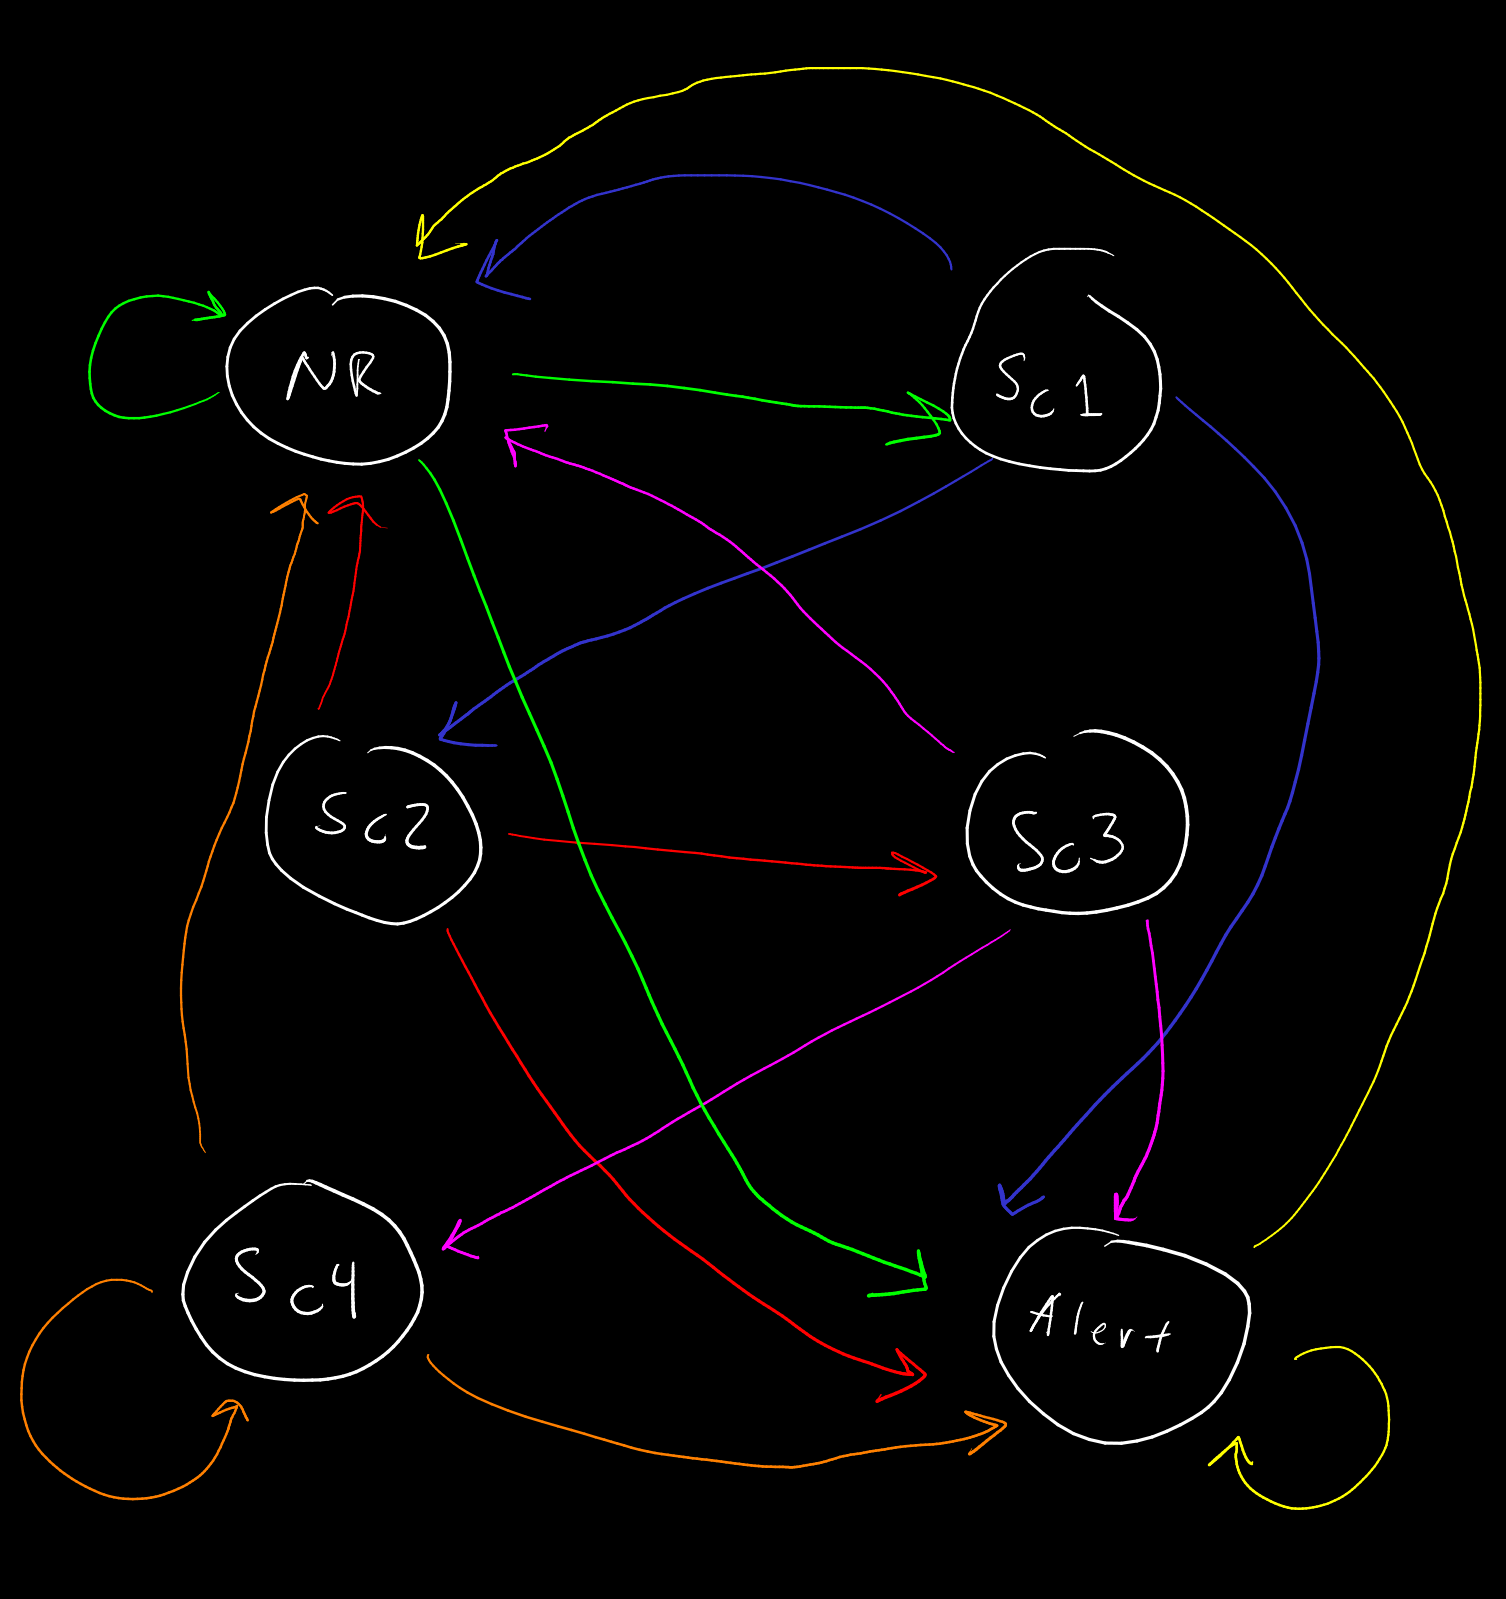
\includegraphics{./grafo1.png}
\caption{Graph for prob.1}
\end{figure}

\newpage

\hypertarget{b}{%
\subsection{b)}\label{b}}

We have first calculated the relative frequencies manually.

\begin{Shaded}
\begin{Highlighting}[]
\KeywordTok{load}\NormalTok{(}\StringTok{'PollutionMadrid.RData'}\NormalTok{)}
\NormalTok{data <-}\StringTok{  }\NormalTok{X[}\DecValTok{1}\NormalTok{,]}
\NormalTok{mat <-}\StringTok{ }\KeywordTok{matrix}\NormalTok{(}\KeywordTok{rep}\NormalTok{(}\DecValTok{0}\NormalTok{,}\DecValTok{36}\NormalTok{), }\DataTypeTok{nrow=}\DecValTok{6}\NormalTok{, }\DataTypeTok{byrow=}\NormalTok{T)}
\ControlFlowTok{for}\NormalTok{ (i }\ControlFlowTok{in} \DecValTok{1}\OperatorTok{:}\KeywordTok{length}\NormalTok{(data)) \{}
  \ControlFlowTok{if}\NormalTok{ (data[i] }\OperatorTok{==}\StringTok{ "Alert"}\NormalTok{) \{}
\NormalTok{    data[i] =}\StringTok{ }\DecValTok{1}
\NormalTok{  \} }\ControlFlowTok{else} \ControlFlowTok{if}\NormalTok{ (data[i] }\OperatorTok{==}\StringTok{ "NR"}\NormalTok{) \{}
\NormalTok{    data[i] =}\StringTok{ }\DecValTok{2}
\NormalTok{  \} }\ControlFlowTok{else} \ControlFlowTok{if}\NormalTok{ (data[i] }\OperatorTok{==}\StringTok{ "Sc1"}\NormalTok{) \{}
\NormalTok{    data[i] =}\StringTok{ }\DecValTok{3}
\NormalTok{  \} }\ControlFlowTok{else} \ControlFlowTok{if}\NormalTok{ (data[i] }\OperatorTok{==}\StringTok{ "Sc2"}\NormalTok{) \{}
\NormalTok{    data[i] =}\StringTok{ }\DecValTok{4} 
\NormalTok{  \} }\ControlFlowTok{else} \ControlFlowTok{if}\NormalTok{ (data[i] }\OperatorTok{==}\StringTok{ "Sc3"}\NormalTok{) \{}
\NormalTok{    data[i] =}\StringTok{ }\DecValTok{5}
\NormalTok{  \} }\ControlFlowTok{else} \ControlFlowTok{if}\NormalTok{ (data[i] }\OperatorTok{==}\StringTok{ "Sc4"}\NormalTok{) \{}
\NormalTok{    data[i] =}\StringTok{ }\DecValTok{6}
\NormalTok{  \}}
\NormalTok{\}}
\NormalTok{data <-}\StringTok{ }\KeywordTok{as.numeric}\NormalTok{(data)}
\ControlFlowTok{for}\NormalTok{ (i }\ControlFlowTok{in} \DecValTok{1}\OperatorTok{:}\KeywordTok{length}\NormalTok{(data)) \{}
\NormalTok{  mat[data[i],data[i}\OperatorTok{+}\DecValTok{1}\NormalTok{]] =}\StringTok{ }\NormalTok{mat[data[i],data[i}\OperatorTok{+}\DecValTok{1}\NormalTok{]] }\OperatorTok{+}\StringTok{ }\DecValTok{1}
\NormalTok{\}}
\NormalTok{mat[data[}\DecValTok{1460}\NormalTok{],data[}\DecValTok{1}\NormalTok{]] =}\StringTok{ }\NormalTok{mat[data[}\DecValTok{1460}\NormalTok{],data[}\DecValTok{1}\NormalTok{]] }\OperatorTok{+}\StringTok{ }\DecValTok{1}

\NormalTok{tbl <-}\StringTok{ }\KeywordTok{table}\NormalTok{(data)}
\ControlFlowTok{for}\NormalTok{ (i }\ControlFlowTok{in} \DecValTok{1}\OperatorTok{:}\KeywordTok{length}\NormalTok{(tbl)) \{}
\NormalTok{  mat[i,] =}\StringTok{ }\NormalTok{mat[i,]}\OperatorTok{/}\NormalTok{tbl[i]}
\NormalTok{\}}
\NormalTok{mat}
\end{Highlighting}
\end{Shaded}

\begin{verbatim}
##            [,1]      [,2]       [,3]      [,4]      [,5]      [,6]
## [1,] 0.00000000 1.0000000 0.00000000 0.0000000 0.0000000 0.0000000
## [2,] 0.00000000 0.9529851 0.04701493 0.0000000 0.0000000 0.0000000
## [3,] 0.01587302 0.4920635 0.00000000 0.4920635 0.0000000 0.0000000
## [4,] 0.00000000 0.5806452 0.00000000 0.0000000 0.4193548 0.0000000
## [5,] 0.23076923 0.3846154 0.00000000 0.0000000 0.0000000 0.3846154
## [6,] 0.00000000 0.5555556 0.00000000 0.0000000 0.0000000 0.4444444
\end{verbatim}

\newpage

We then tested using the \emph{markovchain} package in order to confirm
our results.

\begin{Shaded}
\begin{Highlighting}[]
\NormalTok{data <-}\StringTok{ }\NormalTok{X[}\DecValTok{1}\NormalTok{,]}
\KeywordTok{markovchainFit}\NormalTok{(data)}\OperatorTok{$}\NormalTok{estimate}
\end{Highlighting}
\end{Shaded}

\begin{verbatim}
## MLE Fit 
##  A  6 - dimensional discrete Markov Chain defined by the following states: 
##  Alert, NR, Sc1, Sc2, Sc3, Sc4 
##  The transition matrix  (by rows)  is defined as follows: 
##            Alert        NR        Sc1 Sc2       Sc3       Sc4
## Alert 0.00000000 1.0000000 0.00000000 0.0 0.0000000 0.0000000
## NR    0.00000000 0.9529851 0.04701493 0.0 0.0000000 0.0000000
## Sc1   0.01612903 0.4838710 0.00000000 0.5 0.0000000 0.0000000
## Sc2   0.00000000 0.5806452 0.00000000 0.0 0.4193548 0.0000000
## Sc3   0.23076923 0.3846154 0.00000000 0.0 0.0000000 0.3846154
## Sc4   0.00000000 0.5555556 0.00000000 0.0 0.0000000 0.4444444
\end{verbatim}

~

\hypertarget{what-can-you-say-of-the-comparison-of-your-estimates-andthe-possible-transitions-between-states-that-you-had-argued-in-part-a}{%
\subsubsection{What can you say of the comparison of your estimates
andthe possible transitions between states that you had argued in part
a}\label{what-can-you-say-of-the-comparison-of-your-estimates-andthe-possible-transitions-between-states-that-you-had-argued-in-part-a}}

According to our probabilities shown in the graph. There are 3 arrows
with probability 0. This is due to the fact that in the data there are
zero transitions from \(Sc2 \rightarrow Alert\),
\(Sc4 \rightarrow Alert\), \(NR \rightarrow Alert\),
\(Alert \rightarrow Alert\).

This is logical given that it is very unlikely to hit an alert state.
Unlike the rest of the states.

Later it will be shown that there's a unique stationary distribution
(see 1d).

\begin{figure}
\centering
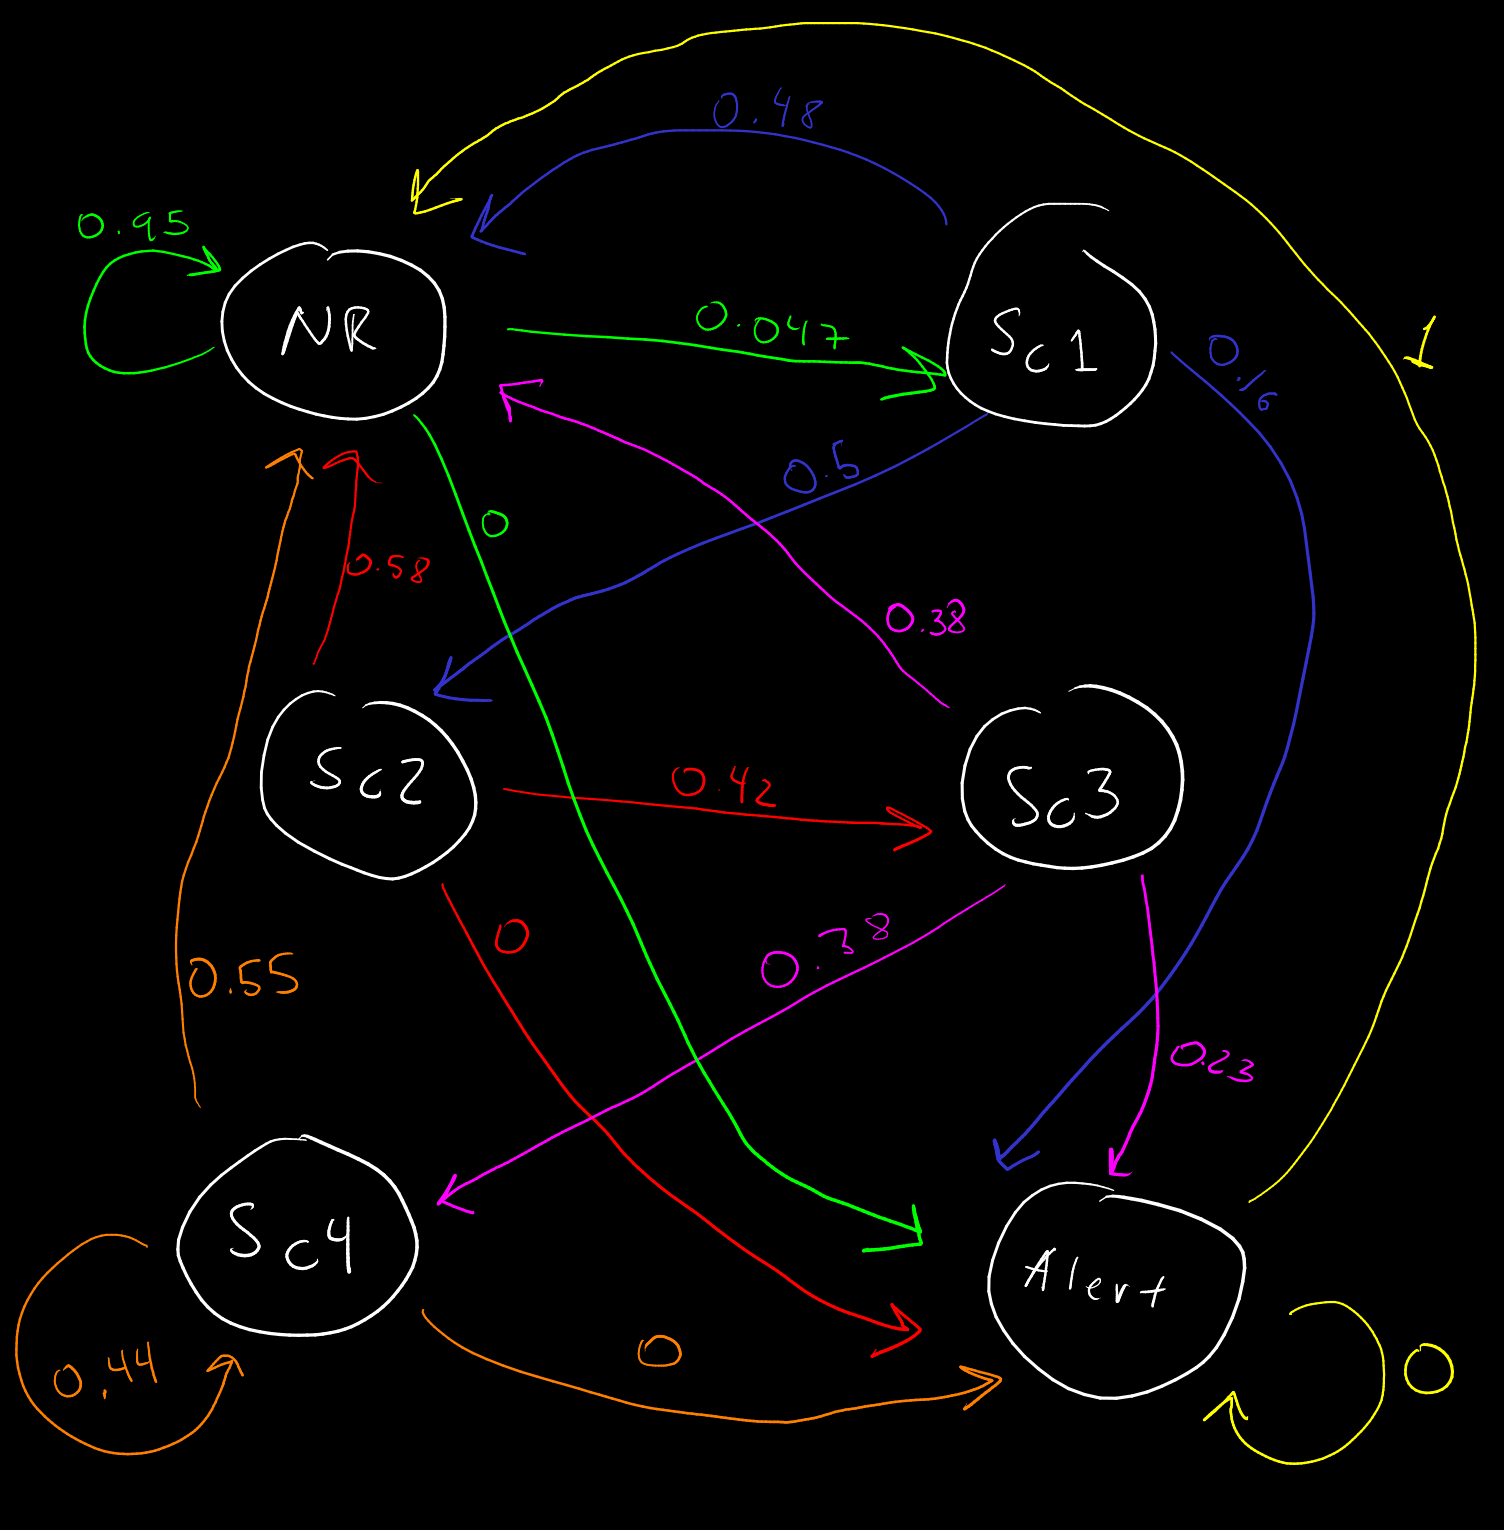
\includegraphics{./grafo1_probs.png}
\caption{Graph with probabilities for problem 1 (b)}
\end{figure}

\newpage

\hypertarget{c}{%
\subsection{c)}\label{c}}

Given that the first state of the chain is NR. We see the following 7
states:

\begin{Shaded}
\begin{Highlighting}[]
\NormalTok{data[}\DecValTok{1}\OperatorTok{:}\DecValTok{7}\NormalTok{]}
\end{Highlighting}
\end{Shaded}

\begin{verbatim}
## [1] "NR" "NR" "NR" "NR" "NR" "NR" "NR"
\end{verbatim}

And we calculate the probability as follows:

\begin{Shaded}
\begin{Highlighting}[]
\NormalTok{mat[}\DecValTok{2}\NormalTok{,}\DecValTok{2}\NormalTok{]}\OperatorTok{^}\DecValTok{7}
\end{Highlighting}
\end{Shaded}

\begin{verbatim}
## [1] 0.713843
\end{verbatim}

We can see the probability is 0.713843

\hypertarget{d}{%
\subsection{d)}\label{d}}

We can see that because we have a unique solution to the system, we have
a unique stationary distribution.

\begin{Shaded}
\begin{Highlighting}[]
\NormalTok{stationary_dist <-}\StringTok{ }\ControlFlowTok{function}\NormalTok{(P) \{}
\NormalTok{    dim =}\StringTok{ }\KeywordTok{sqrt}\NormalTok{(}\KeywordTok{length}\NormalTok{(P))}
\NormalTok{    mat =}\StringTok{ }\KeywordTok{matrix}\NormalTok{(P,}\DataTypeTok{nrow=}\NormalTok{dim, }\DataTypeTok{byrow=}\NormalTok{T)}
\NormalTok{    A =}\StringTok{ }\NormalTok{mat }\OperatorTok{-}\StringTok{ }\KeywordTok{diag}\NormalTok{(dim)}
\NormalTok{    b =}\StringTok{ }\KeywordTok{c}\NormalTok{(}\DecValTok{1}\NormalTok{,}\KeywordTok{rep}\NormalTok{(}\DecValTok{0}\NormalTok{,dim}\DecValTok{-1}\NormalTok{))}
\NormalTok{    A[,}\DecValTok{1}\NormalTok{] <-}\StringTok{ }\KeywordTok{rep}\NormalTok{(}\DecValTok{1}\NormalTok{,dim)}

    \KeywordTok{print}\NormalTok{(}\StringTok{"The solution is the following:"}\NormalTok{)}
\NormalTok{    pi <-}\StringTok{ }\NormalTok{matlib}\OperatorTok{::}\KeywordTok{Solve}\NormalTok{(A, b, }\DataTypeTok{fractions =} \OtherTok{TRUE}\NormalTok{)}
\NormalTok{\}}
\KeywordTok{stationary_dist}\NormalTok{(mat)}
\end{Highlighting}
\end{Shaded}

\begin{verbatim}
## [1] "The solution is the following:"
## x1            =             1/6 
##   x2          =  17201996/66847 
##     x3        =      39543/3224 
##       x4      =         645/104 
##         x5    =        2059/744 
##           x6  =       3725/1681
\end{verbatim}

\hypertarget{e}{%
\subsection{e)}\label{e}}

Taking the 120th power of our transition matrix we get the following:

\begin{Shaded}
\begin{Highlighting}[]
\KeywordTok{matrixpower}\NormalTok{(mat,}\DecValTok{120}\NormalTok{)}
\end{Highlighting}
\end{Shaded}

\begin{verbatim}
##             [,1]      [,2]       [,3]       [,4]       [,5]        [,6]
## [1,] 0.002739726 0.9178082 0.04315068 0.02123288 0.00890411 0.006164384
## [2,] 0.002739726 0.9178082 0.04315068 0.02123288 0.00890411 0.006164384
## [3,] 0.002739726 0.9178082 0.04315068 0.02123288 0.00890411 0.006164384
## [4,] 0.002739726 0.9178082 0.04315068 0.02123288 0.00890411 0.006164384
## [5,] 0.002739726 0.9178082 0.04315068 0.02123288 0.00890411 0.006164384
## [6,] 0.002739726 0.9178082 0.04315068 0.02123288 0.00890411 0.006164384
\end{verbatim}

\newpage

\hypertarget{problem-2}{%
\section{Problem 2}\label{problem-2}}

\hypertarget{a-1}{%
\subsection{a)}\label{a-1}}

We set up the following system of equations:

\(\sum_{i=0} \pi_{i} P_{i,0} = \pi_{1}\)

\(\sum_{i=1} \pi_{i} = 1\)

\((1 - p) \pi_{1} = \pi_{2}\) \(\dots\)
\((1 - p) \pi_{n-2} = \pi_{n-1}\) \(\dots\)

For the first equation, each \(P_{i,0} = p\), therefore:

\(\sum_{i=0} P_{i,0} \pi_{i} = \pi_{1} \Rightarrow p \sum_{i=1} \pi_{i} = \pi_{1}\)

\(p = \pi_{1}\)

\((1 - p)p = \pi_{2}\) \((1 - p)^{2} p = \pi_{3}\) \(\dots\)
\((1 - p)^{n-1} p = \pi_{n}\) \(\dots\)

Then, we get:

Because our MC is an irreducible infinite state MC, we have a unique
stationary distribution \(\pi\), \(\pi_{i} = \frac{1}{\mu_{i}}\) and all
states have expected finite return times then we have:

\(E[T_{i}|X_{0} = i] = \mu_{i} = \frac{1}{\pi_{i}}\)

\hypertarget{b-1}{%
\subsection{b)}\label{b-1}}

Because it has a unique stationary distribution, it can only have one
communication class (it is irreducible), all states are recurring states
and there is no transient state.

\hypertarget{c-1}{%
\subsection{c)}\label{c-1}}

\begin{Shaded}
\begin{Highlighting}[]
\NormalTok{mc <-}\StringTok{ }\ControlFlowTok{function}\NormalTok{(p, sequences ,steps) \{}
\NormalTok{    n <-}\StringTok{ }\DecValTok{100}
\NormalTok{    MarkovChain <-}\StringTok{ }\KeywordTok{matrix}\NormalTok{(}\KeywordTok{rep}\NormalTok{(}\DecValTok{0}\NormalTok{,sequences}\OperatorTok{^}\DecValTok{2}\NormalTok{), }\DataTypeTok{nrow=}\NormalTok{sequences, }\DataTypeTok{byrow=}\OtherTok{TRUE}\NormalTok{)}
\NormalTok{    MarkovChain[,}\DecValTok{1}\NormalTok{] <-}\StringTok{ }\NormalTok{p}
    \ControlFlowTok{for}\NormalTok{ (i }\ControlFlowTok{in} \DecValTok{1}\OperatorTok{:}\NormalTok{sequences) \{}
        \ControlFlowTok{if}\NormalTok{ (i }\OperatorTok{==}\StringTok{ }\NormalTok{sequences) \{}
\NormalTok{            MarkovChain[i,i] <-}\StringTok{ }\DecValTok{0}
\NormalTok{        \} }\ControlFlowTok{else}\NormalTok{ \{}
\NormalTok{            MarkovChain[i,i}\OperatorTok{+}\DecValTok{1}\NormalTok{] <-}\StringTok{ }\DecValTok{1}\OperatorTok{-}\NormalTok{p}
\NormalTok{        \}}
\NormalTok{    \}}
    \KeywordTok{return}\NormalTok{(MarkovChain)}
\NormalTok{\}}
\end{Highlighting}
\end{Shaded}

\end{document}
